% include the figures path relative to the master file
\graphicspath{ {./content/method/figures/} }

\section{Material and Methods}\label{sec:mm}

% Our framework is formulated as a standard classification framework. First the dermoscopy images are represented by a set of elements or features. With reference to our previous studies on melanoma classification \cite{rastgoo2015automatic, rastgoo2015ensemble} the texture and color features with the highest performance are selected. These features include, \Ac{clbp} \cite{guo2010completed}, Gabor filter \cite{Manjunath96-45}, color variance and histogram and hue and opponent angle color histogram \cite{van2006coloring}. The extracted features are explained in the following. The retrieved features are used to train a \Ac{rf} classifier.

\begin{figure*}[Ht]
  \centering
  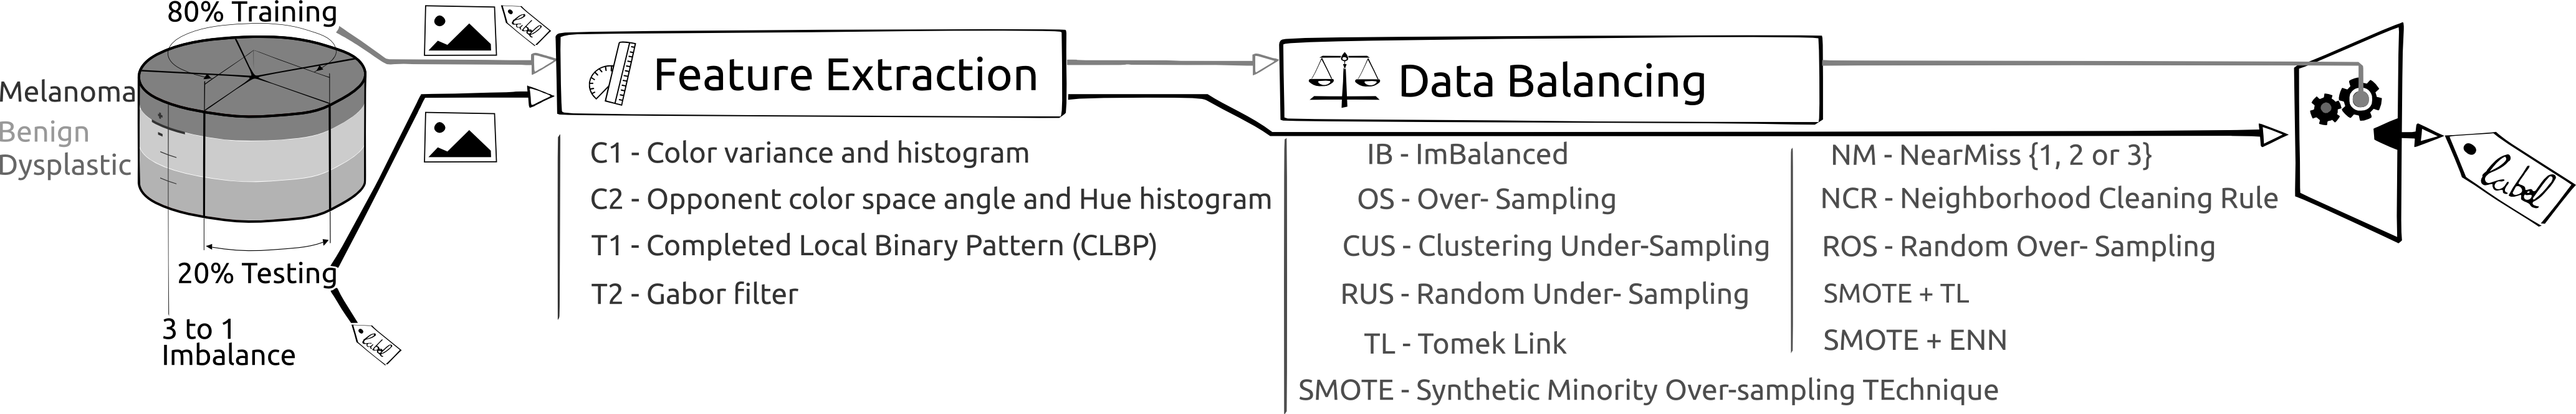
\includegraphics[width=1.\textwidth]{method.png}
  \caption{Framework outline}
	\label{fig:schema}
\end{figure*}

Figure~\ref{fig:schema} illustrates and summarizes the experiment designed to explore the data imbalance problem during the classification of dermoscopic images.
The experimentation is based on the works presented in~\cite{rastgoo2015automatic, rastgoo2015ensemble} and follows a cross-validated classification evaluation framework.
Details of the dataset used for the experiments are given in Sect.\,\ref{sec:dataset}. 
The extracted features correspond to the highest performing subset of features according to the latter mentioned studies and are summarized in Sect.\,\ref{sec:feat}.
The classification is performed using a \ac{rf} classifier with 100 unpruned trees using gini criterion.
The validation model used is a 10-fold cross-validation in which \SI{80}{\percent} of the data are used for training and \SI{20}{\percent} are used for testing.
Furthermore, we dedicate an entire section (see Sect.\,\ref{sec:met}) to focus on the different balancing strategies.

\subsection{Dataset}\label{sec:dataset}
The $PH^{2}$ dermoscopic dataset which is acquired at \textit{Dermatology Service of Hospital Pedro Hispano, Matosinhos, Portugal} is used~\cite{barata2013two}.
The dermoscopic dataset is acquired with Tuebinger Mole Analyzer system with a magnification of $20 \times$.
The 8-bits~RGB color dermoscopic images were obtained under the same conditions with a resolution of $\SI{768}{px} \times \SI{560}{px}$. 
This dataset contains 200 dermoscopic images divided into 160 benign and dysplastic and 40 melanoma lesions. Moreover, each lesion is segmented and histological diagnosis are provided. 
In this study, we conducted the experiments with a subset of 39 melanoma and 117 benign and dysplastic lesions with an imbalance ratio of 1:3.

\subsection{Feature extraction}\label{sec:feat}

\begin{description}
\item[Color variance and histogram ($C_{1}$)] descriptors contain the mean and variance of the nine channels (R, G, B, H, S, V, L, A, B) and the histogram of the R, G and B channels.
\item[Opponent color space angle and Hue histogram ($C_{2}$)] is a robust and rotation invariant feature descriptor derived from the RGB channels~\cite{van2006coloring}:
  \begin{align}\label{Eq:AngO}
    H &= \arctan\left(\frac{\sqrt{3}\left(R-G\right)}{R+G-2B}\right) \ , \nonumber \\
    \theta^{O}_{d} &= \arctan \left( \frac{\sqrt{3}\left(R'_{d}-G'_{d}\right)}{R'_{d}+G'_{d}-2B'_{d}}\right) \ ,
  \end{align}
\noindent where $d$ denotes the spatial coordinates of $(x,y)$ and $R'_{d}$, $G'_{d}$, $B'_{d}$ denote the first order derivatives of RGB channels with respect to the coordinates. 
The color descriptor is built by taking histogram of the opponent angle $\theta^{O}_{d}$ and the hue channel $(H)$.
\item[\ac{clbp} ($T_{1}$)] is a completed modeling of \Ac{lbp}, especially designed for texture classification~\cite{guo2010completed}. 
This descriptor encodes the magnitude and sign differences of the central pixel with its neighbors in the local patterns rather than only the sign differences. 
The \ac{clbp} are calculated for each pixel in a given image and their histogram defines the final descriptor.
\item[Gabor filter ($T_{2}$)] is a linear filter which is defined as a modulation of a Gaussian kernel with a sinusoidal wave. 
This filter is formulated in Eq.\,\eqref{Eq:Gabor} as two Gaussian with standard deviations of $\sigma_{x}$ and $\sigma_{y}$ that vary along $x$ and $y$ axes and it is modulated by a complex sinusoidal with a wavelength of $\lambda$. 
Here $\theta$ represents the orientation of the Gabor filter, $\psi$ is the phase offset and $s$ is the scale factor. 
The filter bank is created using six different orientations equally spaced in the interval $[0, \pi]$, along 4 scales with a downsizing factor of 2:
\begin{equation}\footnotesize
  \label{Eq:Gabor}
  g(x,y) = \exp{ \left(-\left( \frac{x'^{2}}{2\sigma_{x}^{2}}+\frac{y'^{2}}{2\sigma_{y}^{2}} \right) \right)} \cos\left( 2\pi\frac{x'}{\lambda}+\psi \right) \ , 
\end{equation}
\noindent where
%\vspace{-0.1cm}
\begin{align*}
  x' &= s\left( x\cos\theta+y\sin\theta\right) \ ,  \\
  y' &= s\left( -x\sin\theta +y\cos\theta\right) \ .
\end{align*}

\end{description}

% \subsection{validation}

% For evaluation purposes, the results are cross-validated by 10 folds, by splitting 80\% of the data in training and
% the rest for testing. The training set then is balanced using previously described imbalanced techniques. The classification performance are reported in terms of mean \Ac{se}(TPR) and \Ac{sp}(TNR) of 10-fold cross-validation and \Ac{wracc}. The last measure \cite{lavravc1999rule} was defined to eliminate the elements of \ac{se} score which is attributed to chance. In another words this measure considers the bias of the dataset by cooperating the skew ratio $c= \frac{rn}{rp}$ which takes to account the ratio of the two class \cite{powers2011evaluation}. 
% The definition of three aforementioned metrics based on the confusion matrix is explained in \ref{Eq:SESPWRacc}.\\
% %\begin{table}
% %\caption{Confusion matrix    }
% %\centering{
% %\begin{tabular}{ccc}
% %& \multicolumn{2}{c}{Actual}\\
% %\midrule
% %\multicolumn{1}{c|}{\parbox[t]{2mm}{\multirow{2}{*}{\rotatebox[origin=c]{90}{Pred}}}} & TP & FP \\
% %\multicolumn{1}{c|}{}& FN & TN \\
% %\end{tabular}}
% %\end{table}
% {\color{red}{needs probably more alignment}}
% \begin{align}\label{Eq:SESPWRacc}
% \hspace{1.5cm}
% &\begin{tabular}{ccc}
% & \multicolumn{2}{c}{Actual}\\
% \midrule
% \multicolumn{1}{c|}{\parbox[t]{2mm}{\multirow{2}{*}{\rotatebox[origin=c]{90}{Pred}}}} & TP & FP \\
% \multicolumn{1}{c|}{}& FN & TN \\
% \end{tabular} \nonumber \\
% \ac{se} &= \frac{TP}{TP+FN} \nonumber  \hspace{1cm} 
% \ac{sp} =  \frac{TN}{TN+FP} \nonumber \\
% \ac{fpr} &= \frac{FP}{FP+TN} = 1 - \ac{sp} \nonumber \\
% \ac{wracc} &=  \frac{4c(SE+SP-1)}{(1+c)^2}
% \end{align}


%%% Local Variables:
%%% mode: latex
%%% TeX-master: ``../../master''
%%% End:
